%%
%% Copyright 2007, 2008, 2009 Elsevier Ltd
%%
%% This file is part of the 'Elsarticle Bundle'.
%% ---------------------------------------------
%%
%% It may be distributed under the conditions of the LaTeX Project Public
%% License, either version 1.2 of this license or (at your option) any
%% later version.  The latest version of this license is in
%%    http://www.latex-project.org/lppl.txt
%% and version 1.2 or later is part of all distributions of LaTeX
%% version 1999/12/01 or later.
%%
%% The list of all files belonging to the 'Elsarticle Bundle' is
%% given in the file `manifest.txt'.
%%

%% Template article for Elsevier's document class `elsarticle'
%% with numbered style bibliographic references
%% SP 2008/03/01

\documentclass[preprint,10pt,numbers,sort&compress]{elsarticle}

%% Use the option review to obtain double line spacing
%% \documentclass[authoryear,preprint,review,12pt]{elsarticle}

%% Use the options 1p,twocolumn; 3p; 3p,twocolumn; 5p; or 5p,twocolumn
%% for a journal layout:
%% \documentclass[final,1p,times]{elsarticle}
%% \documentclass[final,1p,times,twocolumn]{elsarticle}
%% \documentclass[final,3p,times]{elsarticle}
%% \documentclass[final,3p,times,twocolumn]{elsarticle}
%% \documentclass[final,5p,times]{elsarticle}
%% \documentclass[final,5p,times,twocolumn]{elsarticle}

%% For including figures, graphicx.sty has been loaded in
%% elsarticle.cls. If you prefer to use the old commands
%% please give \usepackage{epsfig}

%% The amssymb package provides various useful mathematical symbols
\usepackage{amssymb}
%% The amsthm package provides extended theorem environments
%% \usepackage{amsthm}

%\usepackage{hyperref}
\usepackage{algorithmicx}
\usepackage[ruled]{algorithm}
\usepackage{algpseudocode}
\usepackage{graphicx}
\usepackage{lineno}
%\usepackage{subfigure} % subfiguras
\usepackage[active]{srcltx}
\usepackage{subcaption}
\usepackage{amssymb}
\usepackage{amsmath}
\usepackage{listings}
\usepackage{color} %red, green, blue, yellow, cyan, magenta, black, white
\definecolor{mygreen}{RGB}{28,172,0} % color values Red, Green, Blue
\definecolor{mylilas}{RGB}{170,55,241}

\allowdisplaybreaks  %Esto es para que permita cambiar de pagina en una formula sin romperla

%% The lineno packages adds line numbers. Start line numbering with
%% \begin{linenumbers}, end it with \end{linenumbers}. Or switch it on
%% for the whole article with \linenumbers.
%% \usepackage{lineno}
\newcommand{\nvidia}{NVIDIA}

\newtheorem{Theorem}{\bf Theorem}[section]
\newtheorem{lemma}{\bf Lemma}%[section]
\newtheorem{definition}{\bf Definition}%[section]
\newtheorem{Corollary}{\bf Corollary}%[section]
\newtheorem{example}{\bf Example}%[section]
\newtheorem{remark}{\bf Remark}%[section]
\newtheorem{proposition}{\bf Proposition}%[section]
\newtheorem{observation}{\bf Note}%[section]
\newtheorem{note}{\bf Note}%[section]
\newproof{pf}{Proof}

\journal{Journal of Computational and Applied Mathematics}

\begin{document}

\lstset{language=Matlab,%
    %basicstyle=\color{red},
    breaklines=true,%
    morekeywords={matlab2tikz},
    keywordstyle=\color{blue},%
    morekeywords=[2]{1}, keywordstyle=[2]{\color{black}},
    identifierstyle=\color{black},%
    stringstyle=\color{mylilas},
    commentstyle=\color{mygreen},%
    showstringspaces=false,%without this there will be a symbol in the places where there is a space
    numbers=left,%
    numberstyle={\tiny \color{black}},% size of the numbers
    numbersep=9pt, % this defines how far the numbers are from the text
    %emph=[1]{for,end,break},emphstyle=[1]\color{red}, %some words to emphasise
    %emph=[2]{word1,word2}, emphstyle=[2]{style},
}
%\linenumbers

\begin{frontmatter}

%% Title, authors and addresses

%% use the tnoteref command within \title for footnotes;
%% use the tnotetext command for theassociated footnote;
%% use the fnref command within \author or \address for footnotes;
%% use the fntext command for theassociated footnote;
%% use the corref command within \author for corresponding author footnotes;
%% use the cortext command for theassociated footnote;
%% use the ead command for the email address,
%% and the form \ead[url] for the home page:
%% \title{Title\tnoteref{label1}}
%% \tnotetext[label1]{}
%% \author{Name\corref{cor1}\fnref{label2}}
%% \ead{email address}
%% \ead[url]{home page}
%% \fntext[label2]{}
%% \cortext[cor1]{}
%% \address{Address\fnref{label3}}
%% \fntext[label3]{}

\title{On Bernoulli matrix polynomials and matrix exponential approximation }

%% use optional labels to link authors explicitly to addresses:
%% \author[label1,label2]{}
%% \address[label1]{}
%% \address[label2]{}

\author[imm]{E.~Defez}
\ead{edefez@imm.upv.es}
\author[i3m]{J. Ib\'a\~nez}
\ead{jjibanez@dsic.upv.es}
\author[dsic]{P. Alonso-Jord\'{a}\corref{cor1}}
\ead{palonso@upv.es}
\author[i3m]{Jos\'e M. Alonso}
\ead{jmalonso@dsic.upv.es}
\author[dsic]{J. Peinado}
\ead{jpeinado@dsic.upv.es}

\address[imm]{Instituto de Matem\'{a}tica Multidisciplinar}
\address[i3m]{Instituto de Instrumentaci\'{o}n para Imagen Molecular}
\address{Universitat Polit\`{e}cnica de Val\`{e}ncia, Camino de Vera s/n, 46022, Valencia. Spain}
\address[dsic]{Department of Information Systems and Computation}

\cortext[cor1]{Corresponding author}

\begin{abstract}
We present in this paper a new method based on Bernoulli matrix polynomials to approximate the exponential of a matrix. 
The developed method has given rise to two new algorithms whose efficiency and precision are compared to the most efficient implementations that currently exist. For that, a state-of-the-art test matrix battery, that allows deeply exploring the highlights and downsides of each method, has been used. 
Since the new algorithms proposed here do make an intensive use of matrix products, we also provide a GPUs-based implementation that allows to achieve a high performance thanks to the optimal implementation of matrix multiplication available on these devices.
\end{abstract}

\begin{keyword}
%% keywords here, in the form: keyword \sep keyword

%% PACS codes here, in the form: \PACS code \sep code

%% MSC codes here, in the form: \MSC code \sep code
%% or \MSC[2008] code \sep code (2000 is the default)
 Bernoulli matrix approximation \sep Matrix exponential function \sep GPU computing
\end{keyword}

\end{frontmatter}

%% \linenumbers

%% main text

\section{Introduction}
The computation of matrix functions has received attention in the last years because of its several applications in different areas of science and technology. Of all the matrix functions, the exponential matrix $e^A$, $A \in \mathbb{C}^{r \times r},$ stands out, due both to its applications in the resolution of systems of differential equations and to the difficulties involved in its computation, see~\cite{Vanl75,MoVa78,MoVa03,High08}.

Among the proposed methods for the approximate computation of the exponential matrix, two fundamental ones stand out: those based on rational Pad\'e approximations \cite{BaGr96,DiPa00,AlHi09,High04}, and those based on polynomial approximations, which are either Taylor series developments~\cite{sastre2015new,SIDR11,RSID16,sastre2019boosting} or serial developments of Hermite matrix polynomials  \cite{defez1998some,sastre2011efficient}. In general, polynomial approximations showed to be more efficient than the Pad\'e algorithm in tests because they are more accurate, despite a slightly higher cost in some cases. All these methods use the basic property of \emph{Scaling-Squaring}, based on the relationship
$$
e^{A}=\left(e^{A/2^s} \right)^{2^s}.
$$

Thus, if ${P_m}(X)$ is a matrix polynomial  approximation of $e^A$, then given a matrix $A$ and a scaling factor $s$,   $P_m(A/2^s)$ is an approximation to $e^{A/2^s}$ and
\begin{equation}
\label{Eq_scaling}
e^{A}\approx \left(P_m(A/2^s) \right)^{2^s}.
\end{equation}

Bernoulli polynomials and Bernoulli numbers have been extensively used in several areas of mathematics, as number theory, and they appear in many mathematical formulas, such as the residual term of the Euler-Maclaurian quadrature rule \cite[p. 63]{olver2010nist}, the Taylor series expansion of the trigonometric functions $\tan{(x)}, \csc{(x)}$ and $\cot{(x)}$ \cite[p. 116-117]{olver2010nist} and the Taylor series expansion of the hyperbolic function $\tanh{(x)}$,  \cite[p. 125]{olver2010nist}. They are also employed in the well known exact expression  of the  even values of the Riemann zeta function:

$$
\xi(2k)=\sum_{n \geq 1} \frac{1}{n^{2k}}=\frac{(-1)^{k-1}B_{2k}(2\pi)^{2k}}{2(2k)!} , k \geq 1.
$$

Morever, they are even used for solving initial value problems \cite{tohidi2013new}, boundary value problems \cite{islam2013numerical,tohidi2013collocation}, high-order linear and nonlinear Fredholm and Volterra integro-differential equations \cite{bhrawy2012new,tohidi2014numerical}, complex differential equations \cite{toutounian2013collocation} and partial differential equations \cite{tohidi2014convergence,tohidi2016new, toutounian2013new}. An excellent survey about Bernoulli polynomials and its applications can be found in  \cite{kouba2013lecture}. The development of series functions of Bernoulli polynomials has been studied in \cite{costabile2001expansion,costabile2001expansions}.

In this paper, we present a new series development of the exponential matrix in terms of \emph{Bernoulli matrix polynomials} which demonstrates that
the polynomial approximations of the exponential matrix are more accurate and less computationally expensive in most cases than those based on Pad\'{e} approximants. 
We also verify that this new method based on Bernoulli matrix polynomials is a competitive method for the
approximation of the exponential matrix, with a similar computational cost than the Taylor one but, generally, more accurate. 


The organization of the paper is as follows. Section~\ref{sec:Bernoulli} is devoted to Bernoulli polynomials. 
We show how to obtain a series of a matrix exponential in terms of Bernoulli matrix polynomials and how to approach that exponential of a matrix. 
The following section describes the algorithm proposed. 
Tests and comparisons are presented in Section~\ref{sec:tests}. 
We close the document with some conclusion remarks.

\subsection*{Notation}
 Throughout this paper, we denote by $\mathbb{C}^{r \times r}$ the set of all the complex square matrices of size $r$ and by $I$ the identity matrix. A polynomial of degree $m$ means an expression of the form $P_m(t)=a_{m} t^m+a_{m-1}t^{m-1}+\cdots+a_{1}t+a_{0}$, where $t$ is a real variable and $a_j$, for $0\leq j \leq m$, are complex numbers. In this way, we can define the matrix polynomial $P_m(B)$ for $B \in \mathbb{C}^{r \times r}$  as $P_m(B)=a_{m} B^m+a_{m-1}B^{m-1}+\cdots+a_{1}B+a_{0}I$.  As usual, the matrix norm $\left\|\cdots \right\|$ denotes any subordinate matrix norm; in particular $\left\| \cdots \right\|_{1}$ is the usual $1-$norm. Finally, if ${\cal A}(k, m)$ are matrices in $\mathbb{C}^{n \times n}$ for $m\geq 0, k \geq 0$, from \cite{rainville1960special} it follows that

\begin{equation}\label{rainville}
\sum_{m \geq 0} \sum_{k \geq 0} {\cal A}(k, m)=\sum_{m \geq 0} \sum_{k=0}^{m} {\cal A}(k, m-k).
\end{equation}

\section{On Bernoulli matrix polynomials}\label{sec:Bernoulli}
The Bernoulli polynomials $B_n(x)$ are defined in \cite[p.588]{olver2010nist} as the coefficients of the generating function

\begin{equation}\label{Bernoulli1}
g(x, t)= \frac{t e^{tx}}{e^t-1}=\sum_{n \geq 0} \frac{B_n(x)}{n!}t^n  \ , \ |t|<2\pi,
\end{equation}
where $g(x, t)$ is an holomorphic function in $\mathbb{C}$ for the variable $t$ (it has an avoidable singularity in $t=0$). 
Bernoulli polynomials  $B_n(x)$ has the explicit expression

\begin{equation}\label{Bernoulli2}
B_n(x)=\sum_{k=0}^{n} {n \choose k} B_k x^{n-k},
\end{equation}
where the Bernoulli numbers are defined by $B_n=B_n(0)$. Therefore, it follows that the Bernoulli numbers satisfy
\begin{equation}\label{Bernoulli3a}
B_0=1, \; \displaystyle  B_{k}= -\sum_{i=0}^{k-1} {k \choose i} \frac{B_i}{k+1-i}, k \geq 1.
\end{equation}
Note that $ B_{3}=B_{5}=\cdots=B_{2k+1}=0$, for
$k\geq 1$. For a matrix $A \in \mathbb{C}^{r \times r}$ we define the $m-th$ Bernoulli matrix polynomial by the expression

\begin{equation}\label{Bernoulli2matrix}
B_m(A)=\sum_{k=0}^{m} {m \choose k} B_k A^{m-k}.
\end{equation}

Thus, we can now calculate the exact value of $\displaystyle e^{At}\left(\frac{t}{e^t-1}\right)$, where $A \in \mathbb{C}^{r \times r}$.
By using (\ref{rainville}) and (\ref{Bernoulli2matrix}) one gets

%\begin{eqnarray*}
%e^{At}\left( \frac{t}{e^t-1} \right) &=& \left(\sum_{n \geq 0} \frac{A^n}{n!}t^n \right) \left(\sum_{k \geq 0} \frac{B_k}{k!}t^k \right) \\
%&=& \sum_{n \geq 0} \sum_{k \geq 0} \frac{A^n B_k}{n! k!}t^n t^k  \\
%&=& \sum_{n \geq 0}\sum_{k=0}^{n} \frac{B_k}{k!}t^k \frac{A^{n-k}}{(n-k)!}t^{n-k} \\
%&=& \sum_{n \geq 0}\left(\sum_{k=0}^{n}{n \choose k} B_k A^{n-k}
%\right) \frac{t^{n}}{n!}\\
%&=& \sum_{n \geq 0} \frac{ B_n(A) t^{n}}{n!},
%\end{eqnarray*}
\begin{displaymath}
e^{At}\left( \frac{t}{e^t-1} \right) 
= \left(\sum_{n \geq 0} \frac{A^n}{n!}t^n \right) \left(\sum_{k \geq 0} \frac{B_k}{k!}t^k \right) 
= \sum_{n \geq 0} \sum_{k \geq 0} \frac{A^n B_k}{n! k!}t^n t^k. 
\end{displaymath}
Taking into account that 
${\cal A}(k, n) = \frac{A^nB_kt^nt^n}{n!k!}$ from~(\ref{rainville}), we have
\begin{eqnarray*}
e^{At}\left( \frac{t}{e^t-1} \right) 
= \sum_{n \geq 0}\sum_{k=0}^{n} \frac{B_k}{k!}t^k \frac{A^{n-k}}{(n-k)!}t^{n-k} \\
= \sum_{n \geq 0}\left(\sum_{k=0}^{n}{n \choose k} B_k A^{n-k} \right) \frac{t^{n}}{n!}
= \sum_{n \geq 0} \frac{ B_n(A) t^{n}}{n!},
%&=& \sum_{n \geq 0}\sum_{k=0}^{n} \frac{B_k}{k!}t^k \frac{A^{n-k}}{(n-k)!}t^{n-k} \\
%&=& \sum_{n \geq 0}\left(\sum_{k=0}^{n}{n \choose k} B_k A^{n-k}
%\right) \frac{t^{n}}{n!}\\
%&=& \sum_{n \geq 0} \frac{ B_n(A) t^{n}}{n!},
\end{eqnarray*}
where $B_n(A)$ is the $n$-th Bernoulli matrix polynomial defined in~(\ref{Bernoulli2matrix}). In this way, we can use the series expansion

\begin{equation}\label{Bernoulli4}
e^{At} = \left(\frac{e^t-1}{t}\right)\sum_{n \geq 0} \frac{ B_n(A) t^{n}}{n!} \ , \ |t|<2\pi,
\end{equation}
to obtain approximations of the matrix exponential. To do this, let's take $s$ the scaling (to be determined) of the matrix $A$ and take $t=1$ in (\ref{Bernoulli4}). We use the matrix exponential  approximation

\begin{equation}\label{Bernoulli5}
e^{A 2^{-s}}\approx  P_{m}(A2^{-s})=\left(e-1 \right)\sum_{n=0}^m \frac{B_n\left(A 2^{-s}\right)}{n!}.
\end{equation}


Approximation (\ref{Bernoulli5}) has the problem that it is not expressed in explicit terms of powers of the matrix $A2^{-s}$. We are going to find that explicit relationship. From
(\ref{Bernoulli5}) we have that, for $m=2$ and using (\ref{Bernoulli2matrix}), one gets



$$
\frac{1}{\left(e-1 \right)}e^{A 2^{-s}}
$$
\begin{eqnarray*}
 & \approx & \sum_{n=0}^2 \frac{B_n\left(A 2^{-s}\right)}{n!} \\
& = & \frac{1}{0!} B_0\left(A 2^{-s}\right) + \frac{1}{1!} B_1\left(A 2^{-s}\right)+ \frac{1}{2!} B_2\left(A 2^{-s}\right) \\
&=& \frac{1}{0!} \left(\sum_{k=0}^{0} {0 \choose k} B_k \left(A 2^{-s}\right)^{0-k} \right) +  \frac{1}{1!} \left(\sum_{k=0}^{1} {1 \choose k} B_k \left(A 2^{-s}\right)^{1-k} \right)\\
&+&  \frac{1}{2!} \left(\sum_{k=0}^{2} {2 \choose k} B_k \left(A 2^{-s}\right)^{2-k} \right) \\
&=& \left(\sum_{k=0}^{2} \frac{1}{k!} {k \choose k} B_k \right) \left(A 2^{-s}\right)^0 + \left(\sum_{k=1}^{2} \frac{1}{k!} {k \choose k-1} B_{k-1} \right) \left(A 2^{-s}\right)^1\\
&+& \left(\sum_{k=2}^{2} \frac{1}{k!} {k \choose k-2} B_{k-2} \right) \left(A 2^{-s}\right)^2.
\end{eqnarray*}

Similarly, for $m=3$:

$$
\frac{1}{\left(e-1 \right)}e^{A 2^{-s}}
$$
\begin{eqnarray*}
& \approx & \sum_{n=0}^3 \frac{B_n\left(A 2^{-s}\right)}{n!} \\
& = & \frac{1}{0!} B_0\left(A 2^{-s}\right) + \frac{1}{1!} B_1\left(A 2^{-s}\right)+ \frac{1}{2!} B_2\left(A 2^{-s}\right)+\frac{1}{3!} B_3\left(A 2^{-s}\right) \\
&=& \frac{1}{0!} \left(\sum_{k=0}^{0} {0 \choose k} B_k \left(A 2^{-s}\right)^{0-k} \right) +  \frac{1}{1!} \left(\sum_{k=0}^{1} {1 \choose k} B_k \left(A 2^{-s}\right)^{1-k} \right)\\
&+&  \frac{1}{2!} \left(\sum_{k=0}^{2} {2 \choose k} B_k \left(A 2^{-s}\right)^{2-k} \right) +  \frac{1}{3!} \left(\sum_{k=0}^{3} {3 \choose k} B_k \left(A 2^{-s}\right)^{3-k} \right)  \\
&=& \left(\sum_{k=0}^{3} \frac{1}{k!} {k \choose k} B_k \right) \left(A 2^{-s}\right)^0 + \left(\sum_{k=1}^{3} \frac{1}{k!} {k \choose k-1} B_{k-1} \right) \left(A 2^{-s}\right)^1 \\
&+& \left(\sum_{k=2}^{3} \frac{1}{k!} {k \choose k-2} B_{k-2} \right) \left(A 2^{-s}\right)^2+\left(\sum_{k=3}^{3} \frac{1}{k!} {k \choose k-3} B_{k-3} \right) \left(A 2^{-s}\right)^3.
\end{eqnarray*}

Taking into account the particular cases $m=2$ and $m=3$, it seems that it is satisfied that

$$
\frac{1}{\left(e-1 \right)}e^{A 2^{-s}} 
$$
\begin{eqnarray}\label{Bernoulli6induccion}
 & \approx & \sum_{n=0}^m \frac{B_n\left(A 2^{-s}\right)}{n!} \nonumber \\
&=& \left(\sum_{k=0}^{m} \frac{1}{k!} {k \choose k} B_k \right) \left(A 2^{-s}\right)^0 + \left(\sum_{k=1}^{m} \frac{1}{k!} {k \choose k-1} B_{k-1} \right) \left(A 2^{-s}\right)^1+\cdots \nonumber \\
&\cdots& + \left(\sum_{k=m}^{m} \frac{1}{k!} {k \choose k-m} B_{k-m} \right) \left(A 2^{-s}\right)^m.
\end{eqnarray}

Let's test the result using induction. Obviously the formula (\ref{Bernoulli6induccion}) is valid for $m=0,1,2,3$. Suppose it is valid for $m$ and let's see for $m+1$. We have


\begin{eqnarray*}
& & \frac{1}{\left(e-1 \right)}e^{A 2^{-s}}  \\
& \approx & \sum_{n=0}^{m+1} \frac{B_n\left(A 2^{-s}\right)}{n!} \\
& = & \sum_{n=0}^{m} \frac{B_n\left(A 2^{-s}\right)}{n!}+\frac{1}{(m+1)!} B_{m+1}\left(A 2^{-s}\right) \\
& = &  \sum_{n=0}^{m} \frac{B_n\left(A 2^{-s}\right)}{n!}+\frac{1}{(m+1)!}\left(  \sum_{k=0}^{m+1} {m+1 \choose k} B_k \left(A 2^{-s}\right)^{m+1-k} \right)\\
&=& \!\!\left(\sum_{k=0}^{m} \frac{1}{k!} {k \choose k} B_k \right)\!\!\left(\!A 2^{-s}\right)^0+\cdots+\!\left(\sum_{k=m}^{m} \frac{1}{k!} {k \choose k\!-\!m} B_{k-m} \right)\!\!\left(\!A 2^{-s}\right)^m\\
&+& \frac{1}{(m+1)!}\left(  \sum_{k=0}^{m+1} {m+1 \choose k} B_k \left(A 2^{-s}\right)^{m+1-k} \right) \\
&=& \left(\sum_{k=0}^{m+1} \frac{1}{k!} {k \choose k} B_k \right)\!\!\left(\!A 2^{-s}\right)^0\!+\!\left(\sum_{k=1}^{m+1} \frac{1}{k!} {k \choose k\!-\!1} B_{k-1} \right)\!\!\left(\!A 2^{-s}\right)^1\!+\cdots \\
&\cdots& +\left(\sum_{k=m+1}^{m+1} \frac{1}{k!} {k \choose k\!-\!(m\!+\!1)} B_{k-(m+1)} \right)\!\!\left(A 2^{-s}\right)^{m+1}.
\end{eqnarray*}

Summarizing we establish the following result:

\begin{Theorem} Given expresion~(\ref{Bernoulli5}), we get
\begin{eqnarray}\label{miaBernoulli1}
\frac{1}{\left(e-1 \right)}e^{\left(A 2^{-s}\right)} &\approx &  \sum_{n=0}^m \frac{B_n\left(A 2^{-s}\right)}{n!}= \sum_{i=0}^m \alpha_{i} \left(A 2^{-s}\right)^{i},
\end{eqnarray}

where $\displaystyle \alpha_{i} = \sum_{k=i}^{m} {k \choose k-i} \frac{B_{k-i}}{k!}$.
\end{Theorem}

\section{The proposed algorithm}\label{sec:algorithm}
To obtain the exponential of matrix $A$ with enough precision and efficiency, it is necessary to determine the values of $m$ and $s$ in  Expression \eqref{Bernoulli5}. Once these values have been determined, the approximation \eqref{Eq_scaling} is used to compute $e^A$. Algorithm \ref{Alg_scaling} computes $e^A$ by using Bernoulli matrix polynomials.

\begin{algorithm}[H]
\caption{Scaling and squaring Bernouilli algorithm for computing $B=e^{A}$,
where $A \in {\mathbb{C}^{r \times r}}$, with $m_{M}$ the maximum approximation order allowed.}
\label{Alg_scaling}
\begin{algorithmic} [1]
\State Choose adequate order $m_k \leqslant {m_{M}}$ and scaling parameter
$s\in \mathbb{N}\cup\{0\}$ for the Bernouilli approximation with scaling.
\State Compute $B = {P_{m_k}}(A/2^{s})$ using (\ref{Bernoulli5})
 \For {$i=1:s$}
    \State $B=B^{2}$
 \EndFor
\end{algorithmic}
\end{algorithm}

As mentioned, in Step 1, the optimal order of the series expansion $m_{k}
\leqslant {m_{M}}$ and the scaling parameter $s$ are chosen. Matrix
polynomial $P_{m}(2^{s}A)$ can be computed optimally in terms of
matrix products using values for $m$ in the set
$m_k=\left\{2,4,6,9,12,16, 20,25,30,\ldots\right\}$,
$k=0,1,\ldots$, respectively, see \cite[p. 72--74]{High08}.

The Bernoulli polynomial coefficients $B_m(A)$, given in~\eqref{Bernoulli2matrix}, differ significantly from those of the Taylor approximation when $m \in \left\{ {2, 4, 6, 9, 12, 16, 20} \right\}$. However, they are practically identical for $m \in \left\{ {25,30} \right\}$. This is because, as the degree of the Bernoulli polynomial increases, all its coefficients vary, approaching the corresponding Taylor ones.

More in detail, the differences in absolute value between the Bernoulli and Taylor series coefficients, when $m = 25$ or $m=30$, are approximately equal or less than the unit roundoff in IEEE double precision $u=2^{-54}\backsimeq 1.11\times 10^{-16}$). For
example, for $m=25$ the difference between the coefficients of the terms of degree 25 has been approximately equal to $1.7431\times10^{-16}$. For the rest of the coefficients, they have been lower than $8.72751\times10^{-17}$, decreasing those values until reaching the lowest value for the coefficient of degree 0 ($4.63073\times10^{-26}$). As expected, for $m = 30$, the differences are smaller than in the previous case, becoming equal to $2.70791\times10^{-33}$ for the term of degree 0. It should be remembered that, in power series of a function, the most significant terms are the first ones.

The algorithm applied in step 1 to calculate $m$ and $s$ is the Algorithm 2 from \cite{RSID16}. In Step 2, we compute the matrix exponential
approximation of the scaled matrix by using the modified Paterson--Stockmeyer's method proposed in \cite[p.
1836-1837]{SIDR11b}:
{\setlength\arraycolsep{2pt}{%\small
\begin{align} \label{PS1}
P_{m_k}(A) & =  \\ ((( p_{m_k}A^q & +  p_{m_k-1}A^{q-1}
+ p_{m_k-2}A^{q-2}   + \dots + p_{m_k-q+1}A  + p_{m_k-q} I ) A^q \nonumber \\ 
\nonumber
               & +  p_{m_k-q-1}A^{q-1} + p_{m_k-q-2}A^{q-2} + \dots + p_{m_k-2q+1}A + p_{m_k-2q} I ) A^q \\ \nonumber
               & +  p_{m_k-2q-1}A^{q-1} + p_{m_k-2q-2}A^{q-2} + \dots + p_{m_k-3q+1}A + p_{m_k-3q} I ) A^q \\ \nonumber
               & \dots  \\ \nonumber
               & +  p_{q-1}A^{q-1} + p_{q-2}A^{q-2} + \dots + p_{1}A + p_{0} I.
\end{align}}
}
Taking into account Table~4.1 from~\cite{High08}, the computational cost in terms of matrix products of~\eqref{PS1} is $k$. 
Finally, in steps $3-5$, the approximation of $e^{A}$ is recovered by using squaring matrix products.
  
\section{Numerical experiments}\label{sec:tests}
In this section, we firstly compare \texttt{expmber}, the new MATLAB implementation developed in this paper based on Bernoulli approximation, with the functions \texttt{exptaynsv3} \cite{RSID16}, that computes the matrix exponential using Taylor matrix polynomials, and \texttt{expm\_new} \cite{AlHi09} which implements a scaling squaring Pad\'e algorithm to work out the mentioned matrix function. 

Next, we compare \texttt{expmbertay}, the novel function that combines Taylor and Bernoulli approximations, with \texttt{expmber}, \texttt{exptaynsv3} and \texttt{expm\_new}. In \texttt{expmbertay}, the matrix exponential is carried out by means of Taylor series, when $m$ is less than or equal to 20, or Bernoulli series, when $m$ is equal to 25 or 30.

All the computations to obtain the {\it``exact"} matrix exponential function were carried out thanks to MATLAB's Symbolic Math Toolbox with 256 digits of precision, using the \texttt{vpa} (variable-precision arithmetic) function and Algorithm~\ref{Alg_exp_exact}.

\begin{algorithm}[H]
\caption{Computes the {\it``exact''} matrix exponential $B=e^{A}$,
where $A \in {\mathbb{C}^{r \times r}}$, by means of Taylor expansion using vpa MATLAB function with $n$ digits of precision.}
\label{Alg_exp_exact}
\begin{algorithmic} [1]
\If{there exist two consecutive orders $m_{k-1},\;m_{k}\in \left\{ {30,36,42,49,56,64} \right\}$ and integers $1 \le i,j \le 15$ for $s$ such that
 \[\frac{{{{\left\| {B_{{m_{k - 1}}}^{(i)}(n) - B_{{m_{k - 1}}}^{(i - 1)}(n)} \right\|}_1}}}{{{{\left\| {B_{{m_{k - 1}}}^{(i)}(n)} \right\|}_1}}} < u,\] and
\[\frac{{{{\left\| {B_{{m_k}}^{(j)}(n) - B_{{m_k}}^{(j - 1)}(n)} \right\|}_1}}}{{{{\left\| {B_{{m_k}}^{(j)}(n)} \right\|}_1}}} < u,\]
and \[\frac{{{{\left\| {B_{{m_k}}^{(j)}(n) - B_{{m_{k - 1}}}^{(i)}(n)} \right\|}_1}}}{{{{\left\| {B_{{m_k}}^{(j)}(n)} \right\|}_1}}} < u\]
by using Algorithm~\ref{Alg_exp_vpa},}

\Return $B={B_{{m_k}}^{(j)}(n)}$
\Else

\Return \textbf{error} 
\EndIf
\end{algorithmic}
\end{algorithm}

\begin{algorithm}[H]
\caption{Computes $B^{(s)}_{m}(n)=e^{A}$,
where $A \in {\mathbb{C}^{r \times r}}$, by Taylor expansion of order $m$ and parameter scaling $s$ with $n$ digits of precision.}
\label{Alg_exp_vpa}
\begin{algorithmic} [1]

\State Compute $B^{(s)}_{m}(n) = {P_{m}}(A/2^{s})$ using Taylor
expansion of order $m$ with $n$ digits of precision
\For {$i=1:s$}
    \State $B^{(s)}_{m}(n)=[B^{(s)}_{m}(n)]^{2}$
 \EndFor
\end{algorithmic}
\end{algorithm}

\subsection{Experiments description}
The following test battery, composed of three types of different and representative matrices, has been chosen to compare the numerical performance of the above described codes:

\begin{itemize}
        \item[a)]  One hundred diagonalizable  $128 \times 128$ real matrices with 1-norms varying from 2.18 to 207.52. These matrices have the form  $A=VDV^T$, where $D$ is a diagonal matrix with real and complex eigenvalues and $V$ is an
        orthogonal matrix obtained as $V=H/\sqrt{128}$, being $H$ the Hadamard matrix.
        The {\it``exact"} matrix exponential was computed as $\exp(A)=V\exp(D)V^T$ (see \cite[pp. 10]{High08}).         

        \item[b)] One hundred non-diagonalizable $128 \times 128$ complex matrices with 1-norms ranging from 84 to 98. These matrices have the form $A=VJV^T$, where $J$ is a Jordan matrix with complex eigenvalues of modulus less than 10 and random algebraic multiplicity varying from 1 to 5. $V$ is an orthogonal matrix obtained as $V=H/\sqrt{128}$, where $H$ is the Hadamard matrix.
        The {\it``exact"} matrix exponential was worked out as $\exp(A)=V\exp(J)V^T$.         
        \item[c)] State-of-the-art matrices:\begin{itemize}
        \item Forty $128 \times 128$ matrices from the Matrix Computation Toolbox (MCT) ~\cite{higham1995test}.
        \item Sixteen matrices from the Eigtool MATLAB package (EMP)~\cite{wrighteigtool} with sizes $127 \times 127$ and $128 \times 128$.
        
                         The {\it``exact"} matrix exponential for these matrices was computed by using Taylor approximations of orders 30, 36, 42, 49, 56 and 64, changing their scaling parameter (see Algorithm~\ref{Alg_exp_exact}).         
        
                 Although the MCT and the EMP are initially composed of fifty-two and twenty matrices, respectively, twelve from the MCT and four from the EMP matrices were discarded for different reasons. For example, matrices 5, 10, 16, 17, 21, 25, 26, 42, 43, 44 and 49 belonging to the MCT and matrices 5 and 6 appertaining to the EMP were not taken into account since the exact exponential solution could not be computed. Besides, matrix 2 from the MCT and matrices 3 and 10 from the EMP were not considered because the excessively high relative error provided by all the methods to be compared.   
\end{itemize}         
       
\end{itemize}

An experiment, called Test, is performed for each of the three sets of matrices described, respectively, 
that evaluates the computational cost and the numerical accuracy of the methods under comparison. 
The three tests have been executed using MATLAB (R2018b) running on an HP Pavilion dv8 Notebook PC with an Intel Core i7 CPU Q720 @1.60Ghz processor and 6 GB of RAM. 

\subsection{Experimental results}

Table \ref{table_prod_comparative} shows the computational costs of each method represented in terms of the number of matrix products (\texttt{P}), taking into account that the cost of the rest of the operations is negligible compared to it for big enough matrices. As it can be seen, \texttt{expmber} and \texttt{exptaynsv3} achieve identical number of matrix multiplications, since the same algorithm was used by both of them to calculate the degree of the polynomial ($m$) and the value of the scaling ($s$). This number of products was lower than that required by \texttt{expm\_new}, which gave rise to the highest computational cost. In addition to the matrix products, \texttt{expm\_new} solves a system of linear equations with $n$ right-hand side vectors where $n$ represents the size of the square coefficient matrix, whose computational cost was approximated as 4/3 matrix products.

%%% Tables products
\begin{table}[!t]\begin{center}
        \caption{Matrix products (P) for  Tests 1, 2 and 3 using \texttt{expmber}, \texttt{exptaynsv3}
and \texttt{expm\_new} MATLAB codes.}
{\footnotesize
        \begin{tabular}{|c||c|c|c|}\hline&\texttt{P(expmber)}&\texttt{P(exptaynsv3)}&\texttt{P(expm\_new)}\\\hline
            Test 1 & 1131 & 1131 & 1178.33 \\\hline
            Test 2 & 1100 & 1100 & 1227.33 \\\hline
            Test 3 & 617  & 617  & 654.67 \\\hline
        \end{tabular}
}
        \label{table_prod_comparative}
    \end{center}
\end{table} 

% Sin tantas líneas 
%\begin{table}[!t]\begin{center}
%        \caption{Matrix products (P) for  Tests 1, 2 and 3 using \texttt{expmber}, \texttt{exptaynsv3}
%and \texttt{expm\_new} MATLAB codes.}
%{\footnotesize
%        \begin{tabular}{ c  c c c }&
%            \texttt{P(expmber)}&\texttt{P(exptaynsv3)}&\texttt{P(expm\_new)}\\\hline
%            Test 1 & 1131 & 1131 & 1178.33 \\
%            Test 2 & 1100 & 1100 & 1227.33 \\
%            Test 3 & 617  & 617  & 654.67 \\\hline
%        \end{tabular}
%}
%        \label{table_prod_comparative}
%    \end{center}
%\end{table} 

Table \ref{table_err_comparative}, on the other hand, shows the percentage of cases in which the relative errors of \texttt{expmber} are lower, greater or equal than those of \texttt{exptaynsv3} and \texttt{expm\_new}. More in detail, the relative error was computed as
$$
\textmd{E}=\frac{\| \exp(A)-\tilde {exp}(A)\|_1}{\left\Vert
\exp(A)\right\Vert_1}
$$where $\tilde {exp}(A)$ is the approximate solution and $\exp(A)$ is the exact one.    

%%%% Tables error
% Table tests 
\begin{table}[!t]\begin{center}
                \caption{Relative error comparison among  \texttt{expmber}
vs  \texttt{exptaynsv3} and  \texttt{expmber}
vs  \texttt{expm\_new} for the three tests.}
{\footnotesize

               \begin{tabular}{|c||c|c|c|}\hline & Test 1  &Test 2 & Test 3\\\hline
                        E(\texttt{expmber})$<$E(\texttt{exptaynsv3})     & 56\% &  91\% & 30.36\%\\\hline
                        E(\texttt{expmber})$>$E(\texttt{exptaynsv3})     & 43\% &   9\%  & 62.5\%\\\hline
                        E(\texttt{expmber})$=$E(\texttt{exptaynsv3})     &  1\%  &   0\%  & 7.14\%\\\hline
                        E(\texttt{expmber})$<$E(\texttt{expm\_new})    & 97\% & 100\% & 69.64\%\\\hline
                        E(\texttt{expmber})$>$E(\texttt{expm\_new})    &   3\% &    0\% & 30.36\%\\\hline
                        E(\texttt{expmber})$=$E(\texttt{expm\_new})    &   0\% &    0\% &       0\%\\\hline
                \end{tabular}
}
                \label{table_err_comparative}
        \end{center}
\end{table}

With the exception of Test 3, the Bernoulli approach resulted in relative errors lower than those of Taylor one. With regard to Pad\'e, the Bernoulli algorithm always offered considerably more accurate results, which reached up to 100\% of the matrices for Test 2.

For the three tests, respectively, the normwise relative errors (a), the performance profiles (b), the ratio of the relative errors (c) and the ratio of the matrix products (d) among the distinct compared methods have been plotted in Figures~\ref{fig:test1},~\ref{fig:test2}, and~\ref{fig:test3}.

\begin{figure}[t]
\centering
\begin{subfigure}[b]{0.48\textwidth}
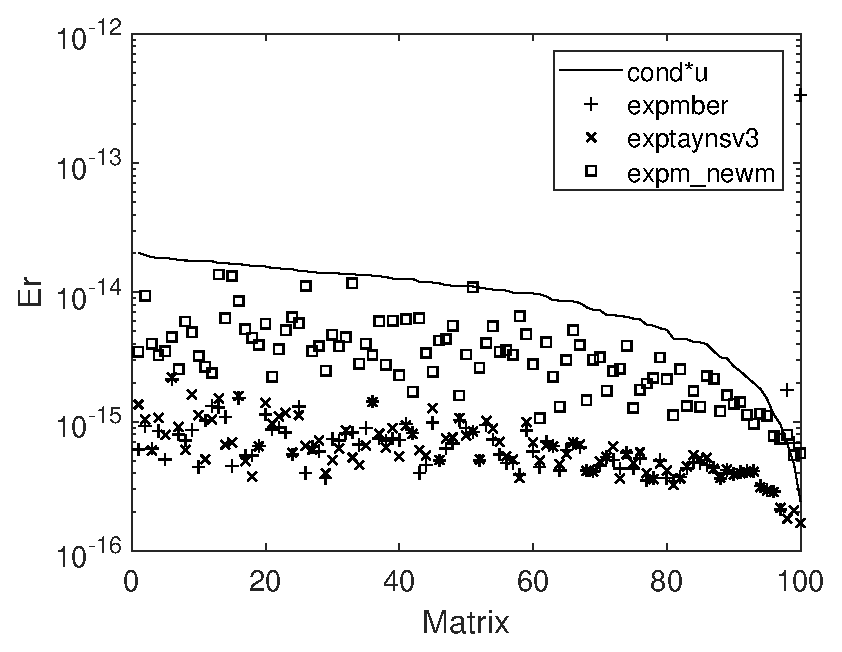
\includegraphics[scale=0.44]{Figures/normwise_exp_diag_hadamard_complex_n128_nd256_expmber.eps}
\caption{\footnotesize Normwise relative errors.} \label{fig:test1_a} \vspace{12pt}
\end{subfigure} \ \
\begin{subfigure}[b]{0.48\textwidth}
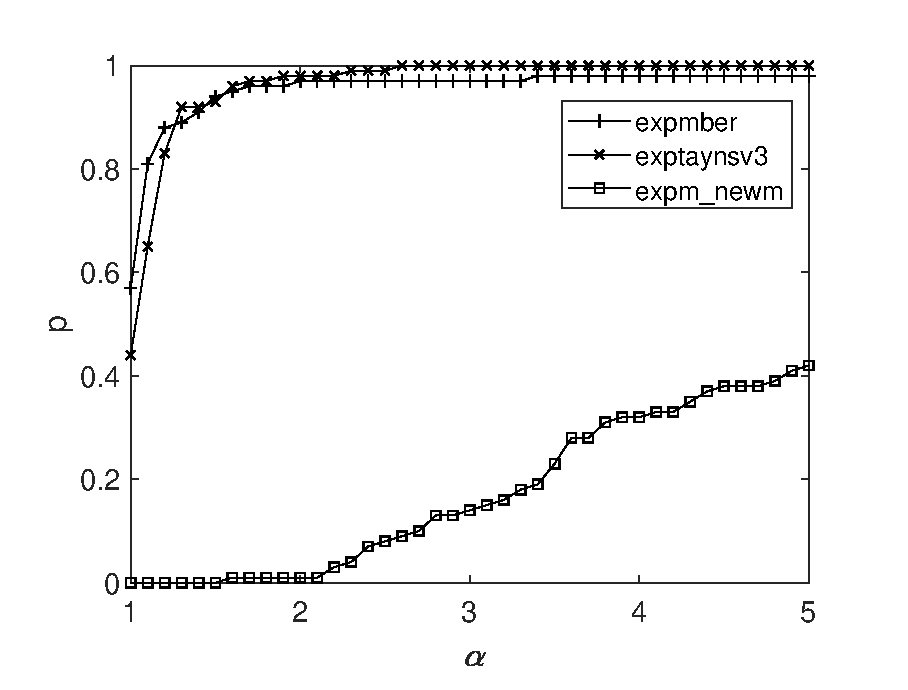
\includegraphics[scale=0.44]{Figures/nprofile_exp_diag_hadamard_complex_n128_nd256_expmber.eps}
\caption{\footnotesize Performance profile.}
\label{fig:test1_b}
\vspace{12pt}
\end{subfigure}
\begin{subfigure}[b]{0.48\textwidth}
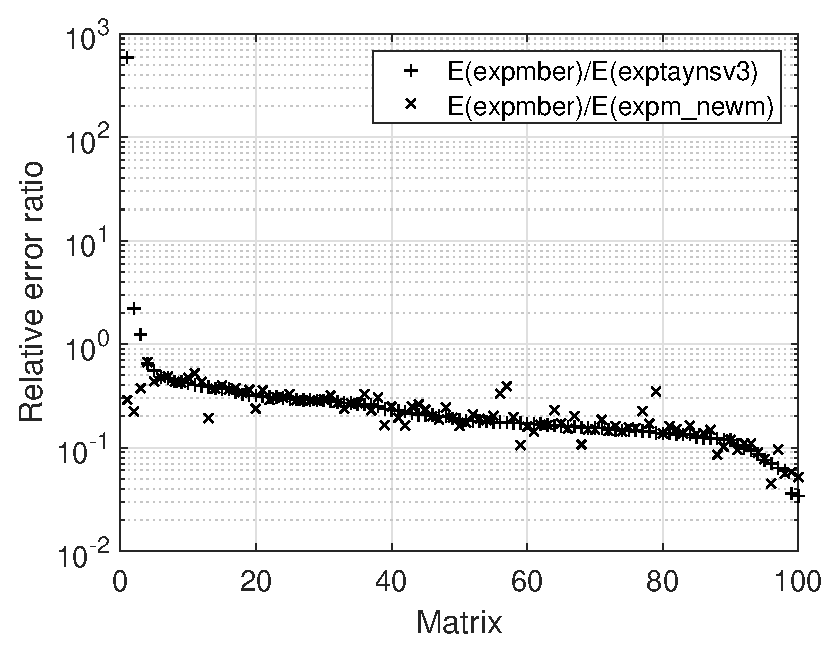
\includegraphics[scale=0.44]{Figures/error_ratio_exp_diag_hadamard_complex_n128_nd256_expmber.eps}
\caption{\footnotesize Ratio of relative errors.}
\label{fig:test1_c}
\end{subfigure}
\begin{subfigure}[b]{0.48\textwidth}
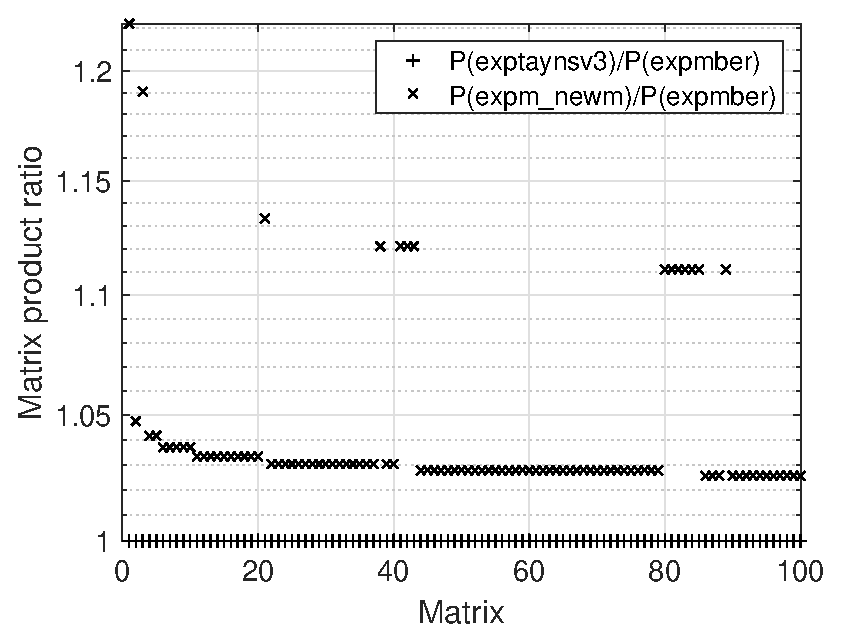
\includegraphics[scale=0.44]{Figures/matrix_product_ratio_exp_diag_hadamard_complex_n128_nd256_expmber.eps}
\caption{\footnotesize Ratio of matrix products.}
\label{fig:test1_d}
\end{subfigure}
\caption{Experimental results for Test~1.}
\label{fig:test1}
\end{figure}
        
\begin{figure}[t]
\centering
\begin{subfigure}[b]{0.48\textwidth}
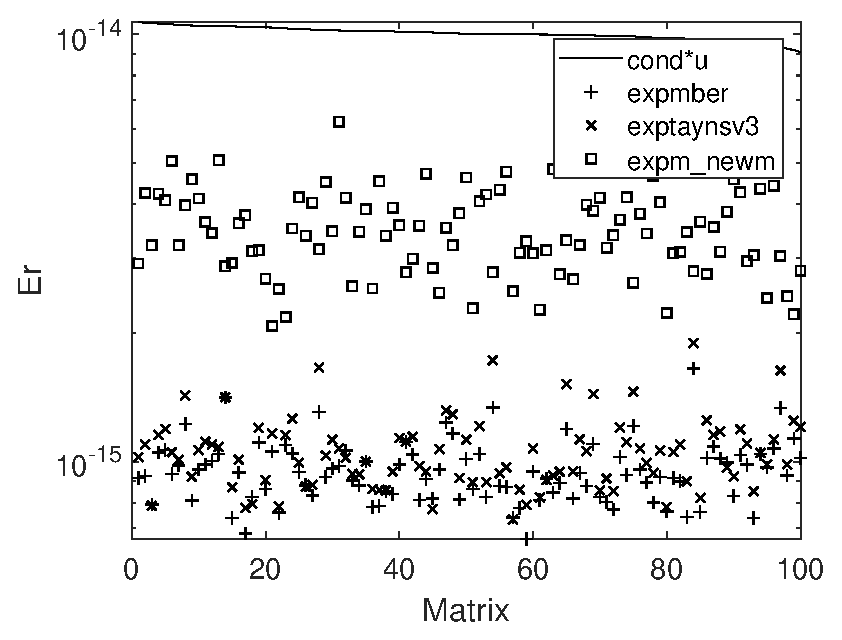
\includegraphics[scale=0.44]{Figures/normwise_exp_jordan_hadamard_complex_n128_boundvp10_maxmult5_nd256_expmber.eps}
\caption{\footnotesize Normwise relative errors.} \label{fig:test2_a} \vspace{12pt}
\end{subfigure} \ \
\begin{subfigure}[b]{0.48\textwidth}
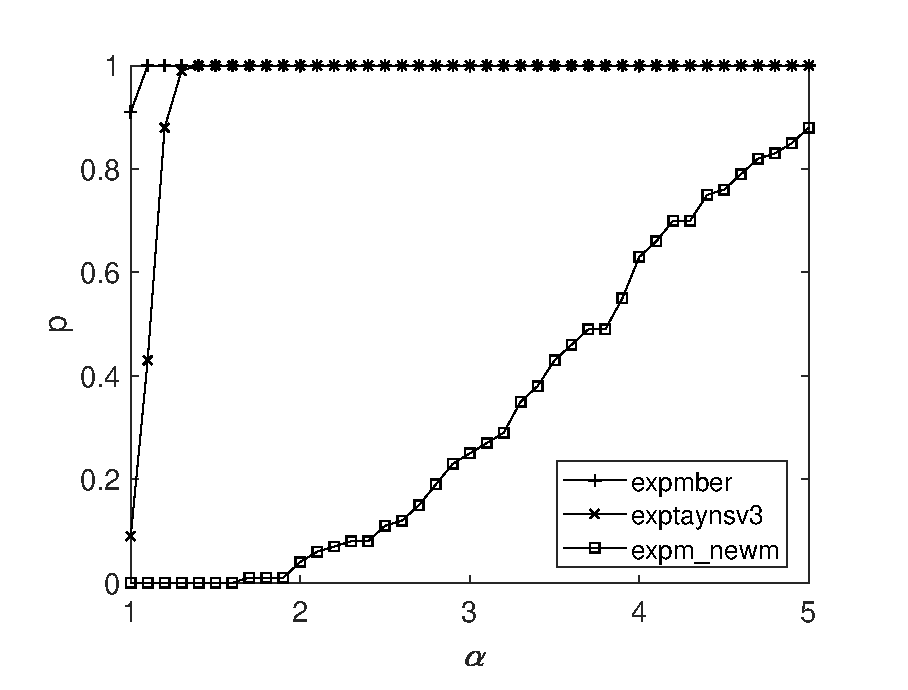
\includegraphics[scale=0.44]{Figures/nprofile_exp_jordan_hadamard_complex_n128_boundvp10_maxmult5_nd256_expmber.eps}
\caption{\footnotesize Performance profile.}
\label{fig:test2_b}
\vspace{12pt}
\end{subfigure}
\begin{subfigure}[b]{0.48\textwidth}
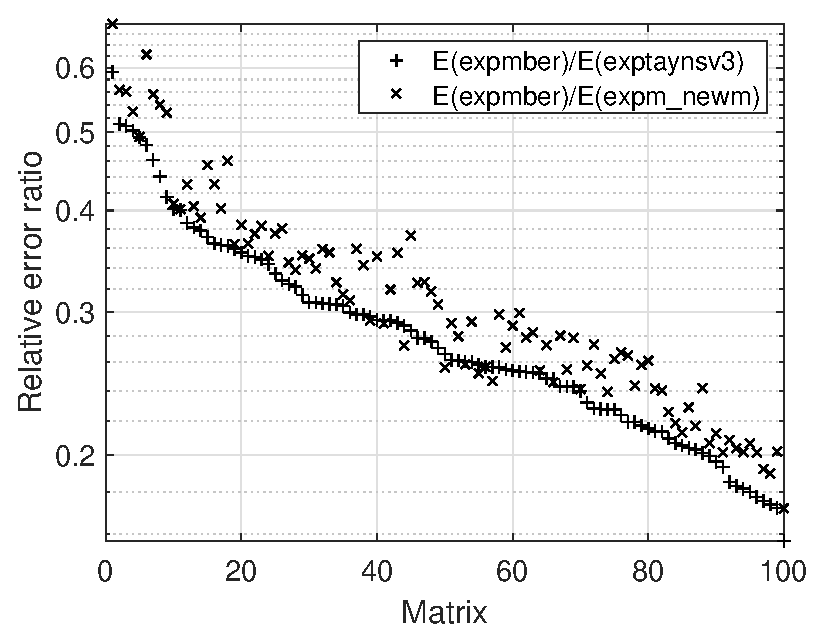
\includegraphics[scale=0.44]{Figures/error_ratio_exp_jordan_hadamard_complex_n128_boundvp10_maxmult5_nd256_expmber.eps}
\caption{\footnotesize Ratio of relative errors.}
\label{fig:test2_c}
\end{subfigure}
\begin{subfigure}[b]{0.48\textwidth}
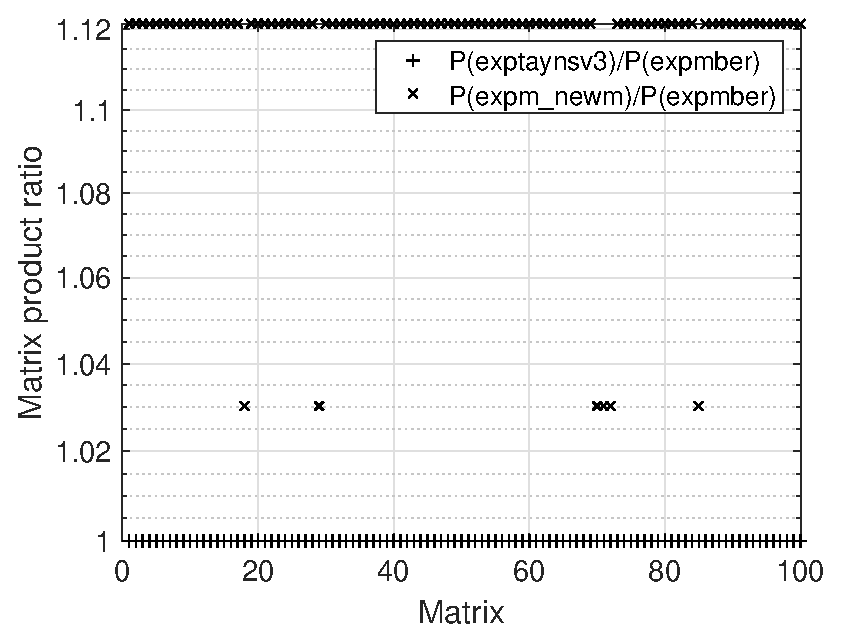
\includegraphics[scale=0.44]{Figures/matrix_product_ratio_exp_jordan_hadamard_complex_n128_boundvp10_maxmult5_nd256_expmber.eps}
\caption{\footnotesize Ratio of matrix products.}
\label{fig:test2_d}
\end{subfigure}
\caption{Experimental results for Test~2.}
\label{fig:test2}
\end{figure}

\begin{figure}[t]
\centering
\begin{subfigure}[b]{0.48\textwidth}
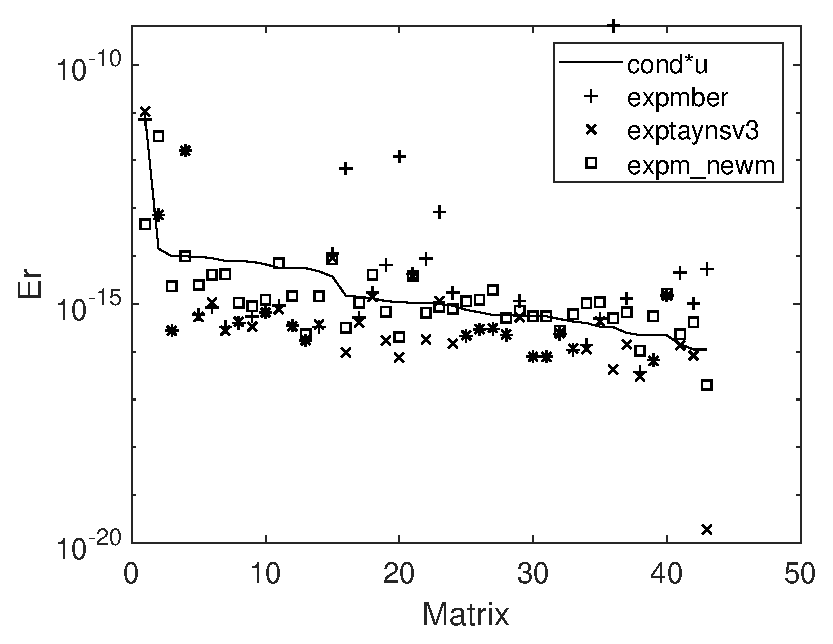
\includegraphics[scale=0.44]{Figures/normwise_exp_toolbox_n128_nd256-exp_eigtool_n128_nd256_expmber.eps}
\caption{\footnotesize Normwise relative errors.} \label{fig:test3_a} \vspace{12pt}
\end{subfigure} \ \
\begin{subfigure}[b]{0.48\textwidth}
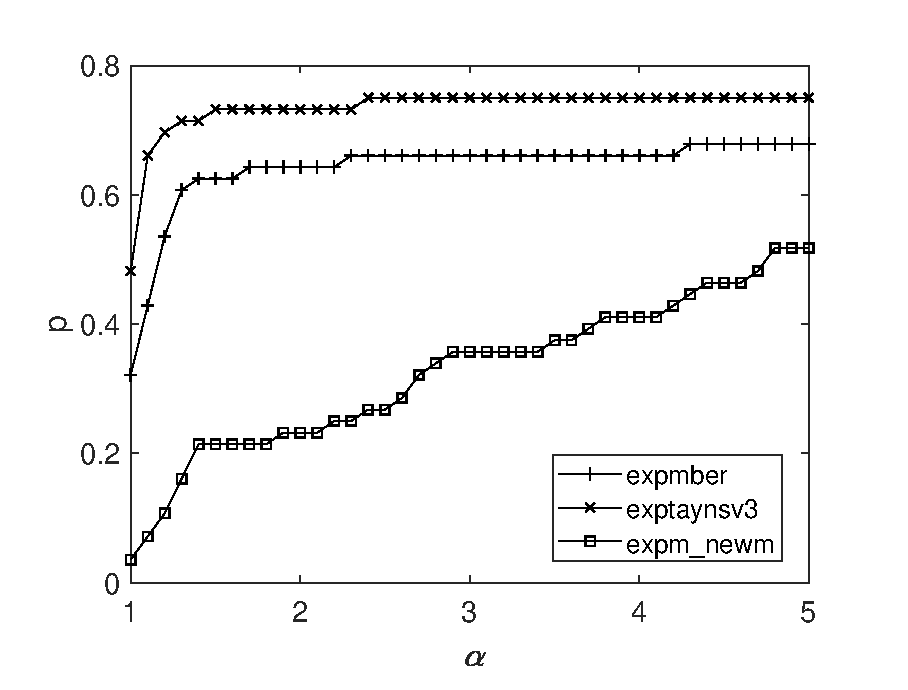
\includegraphics[scale=0.44]{Figures/nprofile_exp_toolbox_n128_nd256-exp_eigtool_n128_nd256_expmber.eps}
\caption{\footnotesize Performance profile.}
\label{fig:test3_b}
\vspace{12pt}
\end{subfigure}
\begin{subfigure}[b]{0.48\textwidth}
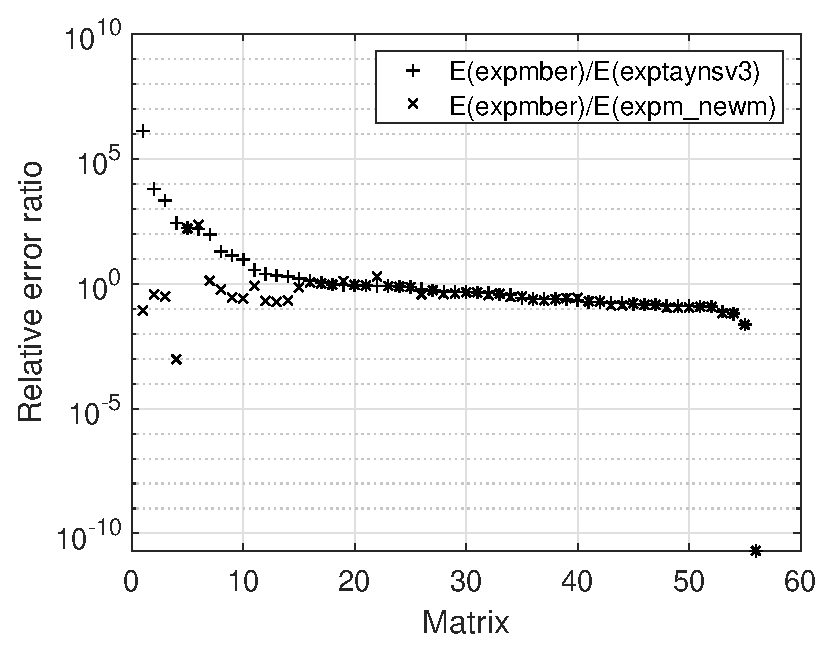
\includegraphics[scale=0.44]{Figures/error_ratio_exp_toolbox_n128_nd256-exp_eigtool_n128_nd256_expmber.eps}
\caption{\footnotesize Ratio of relative errors.}
\label{fig:test3_c}
\end{subfigure}
\begin{subfigure}[b]{0.48\textwidth}
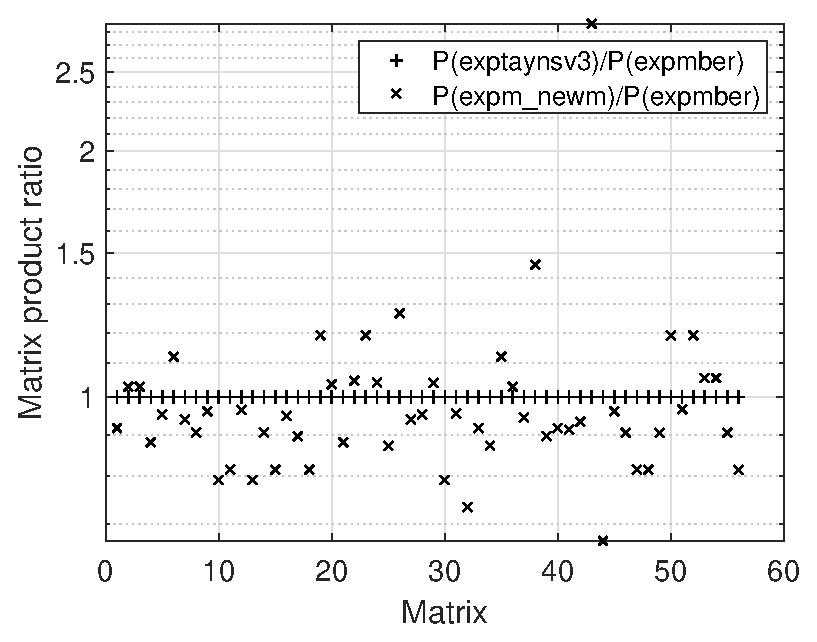
\includegraphics[scale=0.44]{Figures/matrix_product_ratio_exp_toolbox_n128_nd256-exp_eigtool_n128_nd256_expmber.eps}
\caption{\footnotesize Ratio of matrix products.}
\label{fig:test3_d}
\end{subfigure}
\caption{Experimental results for Test~3.}
\label{fig:test3}
\end{figure}

Regarding the normwise relative errors presented in Figures~\ref{fig:test1_a}, \ref{fig:test2_a} and \ref{fig:test3_a}, their solid line represents the function ${k_{\exp}}u$, where ${k_{\exp}}$ (or $cond$) is the condition number of the matrix exponential function \cite[Chapter 3]{High08} and $u=2^{-53}$ is the unit roundoff in the IEEE double precision floating-point arithmetic. In general, \texttt{expmber} exhibited a very good numerical stability. This can be appreciated seeing the distance from each matrix normwise relative error to the $cond*u$ line. In Figures~\ref{fig:test1_a} and \ref{fig:test2_a}, the numerical stability is even much better because these errors are below this line. Because ${k_{\exp}}$ was infinite or enormously high for the matrices 6, 7, 12, 15, 23, 36, 39, 50 and 51 from the MCT and for the matrices 1, 4, 8 and 15 from the EMP, all of them were rejected in the Figure \ref{fig:test3_a} visualisation but considered in the other ones.

In the performance profile Figures (\ref{fig:test1_b}, \ref{fig:test2_b} and \ref{fig:test3_b}), the $\alpha$ coordinate, on the $x$-axis, varies from 1 to 5 in steps equal to 0.1. For a concrete $\alpha$ value, the $p$ coordinate,  on the $y$-axis,  means the probability that the considered algorithm has a relative error lower than or equal to $\alpha$-times the smallest relative error over all the methods on the given test. For the first two tests (Figures~\ref{fig:test1_b}, \ref{fig:test2_b}), the performance profile shows that Bernoulli and Taylor methods accuracy was similar. Both of them had much better correctness than the Pad\'e method. Nothwithstanding, Figure~\ref{fig:test3_b} reveals that \texttt{exptaynsv3} code improved the result accuracy against the \texttt{expmber} function, for the Test 3. 

In Figures \ref{fig:test1_c}, \ref{fig:test2_c} and \ref{fig:test3_c}, the ratios of relative errors have been presented in decreasing order with respect to E(\texttt{expmber})/E(\texttt{exptaynsv3}). They confirm the data exposed in Table \ref{table_err_comparative}, where it was shown that \texttt{expmber} provides more accurate results than \texttt{exptaynsv3} for Tests 1 and 2, but not for Test 3. It is obvious to note that Pade offered the worst performance in most cases.

In our opinion, this is clearly due to the distinctive numerical characteristics of the 3 sets of matrices analysed and the degree of the polynomial ($m$) required to be used. According to our experience, \texttt{expmber} provides results with a very appropriate accuracy for values of $m$ equal to 25 or 30. However, for significantly lower values, \texttt{expmber} will be less competitive than other codes, such as \texttt{exptaynsv3}. Minimum, maximum and average values of $m$ required for Tests 1, 2 and 3 are collected in Table \ref{table_m_comparative}. In more detail, Figure \ref{fig:m_value} shows the approximation polynomial order employed in the calculation of the exponential function by means of \texttt{expmber} (or \texttt{exptaynsv3}) for each of the matrices that are part of the test battery.

%%%% Table degree of polynomial
\begin{table}[!t]\begin{center}
        \caption{Mininum, maximum and average polynomial degree (m) required for Tests 1, 2 and 3 using \texttt{expmber} or \texttt{exptaynsv3} functions.}
{\footnotesize
        \begin{tabular}{|c||c|c|c|}\hline & Minimum & Maximum & Average \\\hline
            Test 1 & 16 & 30 & 27.51 \\\hline
            Test 2 & 30 & 30 & 30 \\\hline
            Test 3 & 12 & 30 & 25.70 \\\hline
        \end{tabular}}
        \label{table_m_comparative}
    \end{center}
\end{table} 


\begin{figure}[t]
\centering
\begin{subfigure}[b]{0.48\textwidth}
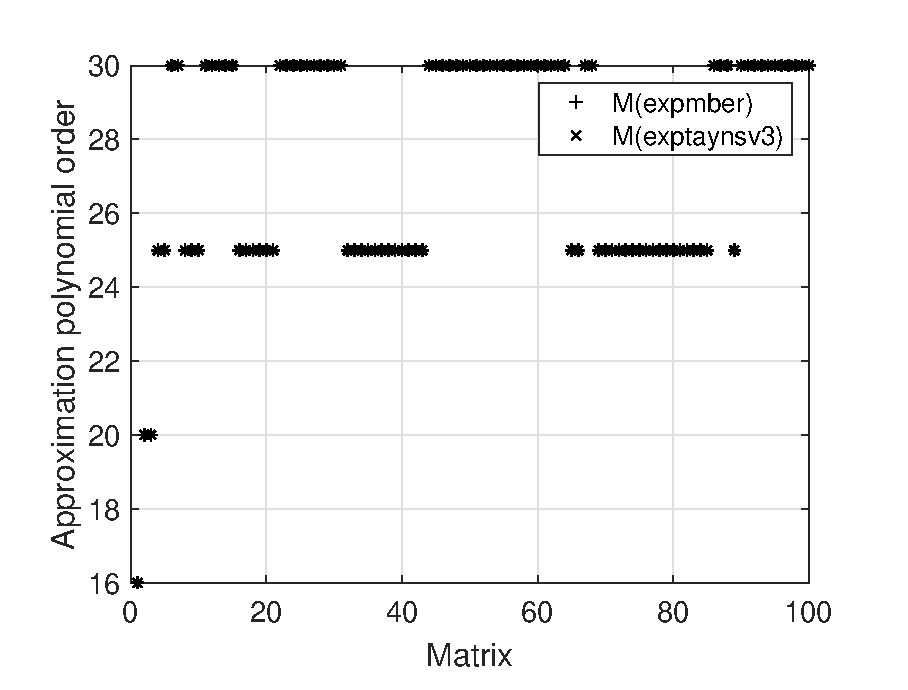
\includegraphics[scale=0.44]{Figures/polynomial_order_exp_diag_hadamard_complex_n128_nd256_expmber.eps}
\caption{\footnotesize Test~1.} \label{fig:m_value_test1} \vspace{12pt}
\end{subfigure} \ \
\begin{subfigure}[b]{0.48\textwidth}
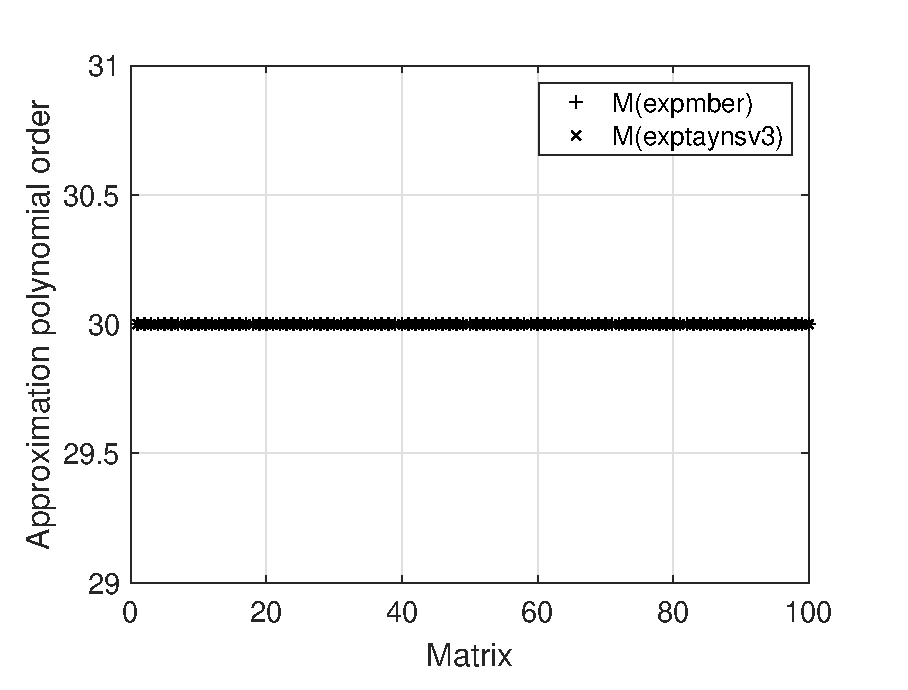
\includegraphics[scale=0.44]{Figures/polynomial_order_exp_jordan_hadamard_complex_n128_boundvp10_maxmult5_nd256_expmber.eps}
\caption{\footnotesize Test~2.}
\label{fig:m_value_test2}
\vspace{12pt}
\end{subfigure}
\begin{subfigure}[b]{0.48\textwidth}
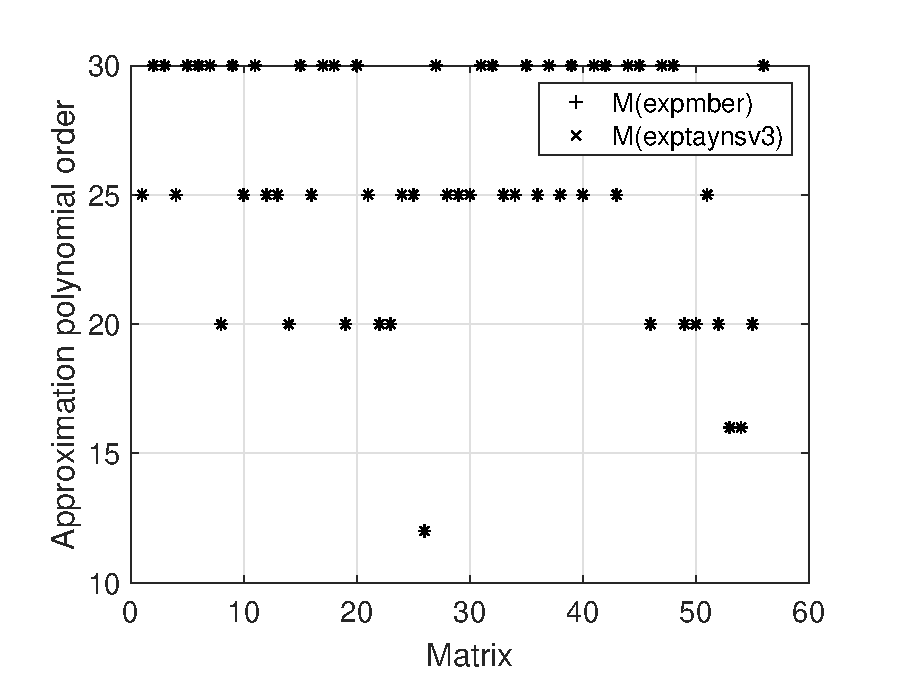
\includegraphics[scale=0.44]{Figures/polynomial_order_exp_toolbox_n128_nd256-exp_eigtool_n128_nd256_expmber.eps}
\caption{\footnotesize Test~3.}
\label{fig:m_value_test3}
\end{subfigure}
\caption{Polynomial order (m) for Test~1, 2 and 3.}
\label{fig:m_value}
\end{figure}

As it was presented in Table \ref{table_prod_comparative}, \texttt{expmber} and \texttt{exptaynsv3} functions performed a lower number of matrix operations than \texttt{expm\_new} one. This statement can be also corroborated from the results displayed in Figures \ref{fig:test1_d}, \ref{fig:test2_d} and \ref{fig:test3_d}, where the ratio between the number of \texttt{expm\_new} and \texttt{expmber} matrix products ranged from 1.03 to 1.22 for Test 1, from 1.03 to 1.12 for Test 2 and from 0.67 to 2.87 for Test 3.

Next, we will analyse the possibility of using Bernoulli and Taylor methods together, giving place to a novel approach to compute the matrix exponential function. For that, we will start getting the benefits of the \texttt{exptaynsv3} function against \texttt{expm\_new} one.  As Table \ref{table_err_comparative_exptaynsv3} shows, the percentage of cases in which Taylor relative error is lower than Pad\'e reaches 100\% for Test 1 and 2, and 89.29\% for Test 3. Evidently, these error percentages improve those offered by Bernoulli approximation with respect to \texttt{expm\_new}, as described in Table \ref{table_err_comparative}. 

%%%% Tables error
% Table tests 
\begin{table}[!t]\begin{center}
                \caption{Relative error comparison between \texttt{exptaynsv3} and \texttt{expm\_new} for the three tests.}
{\footnotesize
               \begin{tabular}{|c||c|c|c|}\hline & Test 1  &Test 2 & Test 3\\\hline
                        E(\texttt{exptaynsv3})$<$E(\texttt{expm\_new})    & 100\% & 100\% & 89.29\%\\\hline
                        E(\texttt{exptaynsv3})$>$E(\texttt{expm\_new})    &   3\% &     0\%  & 10.71\%\\\hline
                        E(\texttt{exptaynsv3})$=$E(\texttt{expm\_new})    &   0\% &     0\%  &       0\%\\\hline
                \end{tabular}}
                \label{table_err_comparative_exptaynsv3}
        \end{center}
\end{table}

From these excellent results, we therefore considered the possibility of combining Bernoulli and Taylor methods, giving rise to the \texttt{expmbertay} code. In this new function, and according to the comparison between the coefficients of their polynomials carried out previously, we will use the Taylor approach (\texttt{exptaynsv3}) for values of m below 25 and the Bernoulli approximation (\texttt{expmber}) when m equals 25 or 30. In this way, the number of matrix products needed by \texttt{expmbertay} will obviously be identical to that of \texttt{expmber} or \texttt{exptaynsv3}. 

Table \ref{table_err_comparative_expmbertay} collects thus the percentage of matrices in which the relative errors of \texttt{expmbertay} are lower, greater or equal than those of \texttt{exptaynsv3}, \texttt{expmber}  and \texttt{expm\_new}.  For the vast majority of matrices, \texttt{expmbertay} provided an accuracy in the results practically identical to that of \texttt{expmber}, but improving even the latter by 23.21\% for the matrices of Test 3. With respect to \texttt{exptaynsv3}, \texttt{expmbertay} also enhanced the results achieved by \texttt{expmber}, so that this combined method is now better or equal than \texttt{exptaynsv3} in 55.36\% of cases for Test 3. Moreover, \texttt{expmbertay} became better than \texttt{expm\_new} in 100\% of the matrices for Test 1 and 2, and 91.07\% for Test 3, which is higher than the percentages individually offered by \texttt{expmber} (69.64\%) and \texttt{exptaynsv3} (89.29\%).

%%%% Tables error
% Table tests 
\begin{table}[!t]\begin{center}
                \caption{Relative error comparison among \texttt{expmbertay} vs \texttt{exptaynsv3}, \texttt{expmbertay} vs \texttt{expmber}, and \texttt{expmbertay} vs \texttt{expm\_new} for the three tests.}
{\footnotesize
               \begin{tabular}{|c||c|c|c|}\hline & Test 1  &Test 2 & Test 3\\\hline
                        E(\texttt{expmbertay})$<$E(\texttt{exptaynsv3})    &   57\%  &   91\%  & 44.64\%\\\hline
                        E(\texttt{expmbertay})$>$E(\texttt{exptaynsv3})    &   42\%  &     9\%  & 44.64\%\\\hline
                        E(\texttt{expmbertay})$=$E(\texttt{exptaynsv3})    &     1\%  &     0\% &  10.72\%\\\hline
                        E(\texttt{expmbertay})$<$E(\texttt{expmber})       &     3\%  &     0\%  & 23.21\%\\\hline
                        E(\texttt{expmbertay})$>$E(\texttt{expmber})       &     0\%  &     0\%  &    0\%\\\hline
                        E(\texttt{expmbertay})$=$E(\texttt{expmber})       &   97\%  &  100\%  & 76.79\%\\\hline
                        E(\texttt{expmbertay})$<$E(\texttt{expm\_new})   & 100\%  & 100\%  &  91.07\%\\\hline
                        E(\texttt{expmbertay})$>$E(\texttt{expm\_new})   &    0\%  &     0\%  &  8.93\%\\\hline
                        E(\texttt{expmbertay})$=$E(\texttt{expm\_new})   &    0\%  &     0\%  &       0\%\\\hline
                \end{tabular}}
                \label{table_err_comparative_expmbertay}
        \end{center}
\end{table}

Numerical features of \texttt{expmbertay} are finally exposed in Figures \ref{fig:test4}, \ref{fig:test5} and \ref{fig:test6} for the three tests by means of the normwise relative errors (a), the performance profiles (b) and the ratio of the relative errors (c). As it can be seen, the method presents an excellent precision in the results, with very low relative errors and a very high probability in the performance profile pictures.
\begin{figure}[t]
\centering
\begin{subfigure}[b]{0.48\textwidth}
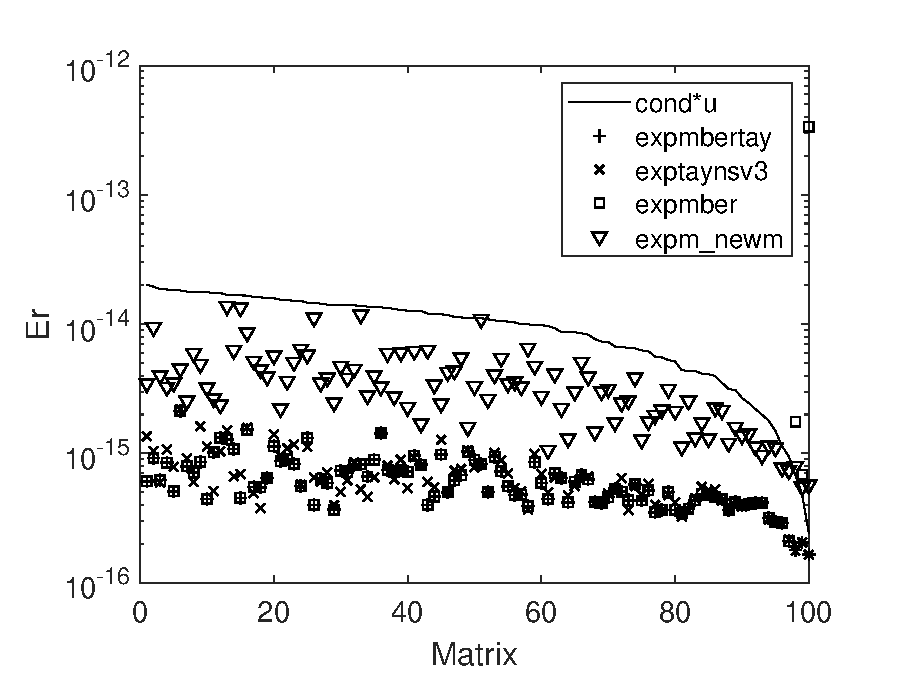
\includegraphics[scale=0.44]{Figures/normwise_exp_diag_hadamard_complex_n128_nd256_expmbertay.eps}
\caption{\footnotesize Normwise relative errors.} \label{fig:test4_a} \vspace{12pt}
\end{subfigure} \ \
\begin{subfigure}[b]{0.48\textwidth}
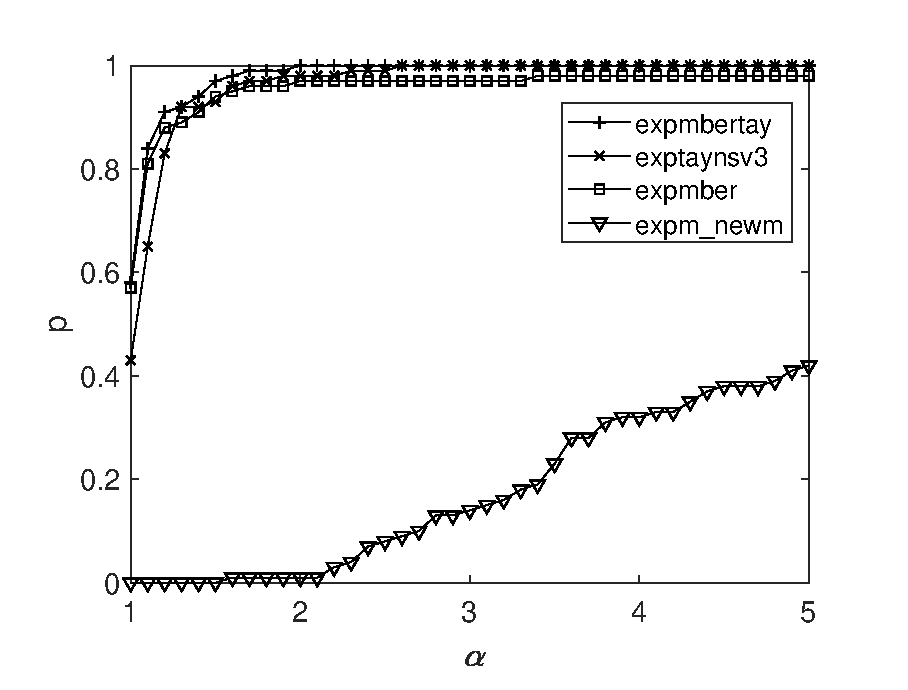
\includegraphics[scale=0.44]{Figures/nprofile_exp_diag_hadamard_complex_n128_nd256_expmbertay.eps}
\caption{\footnotesize Performance profile.}
\label{fig:test4_b}
\vspace{12pt}
\end{subfigure}
\begin{subfigure}[b]{0.48\textwidth}
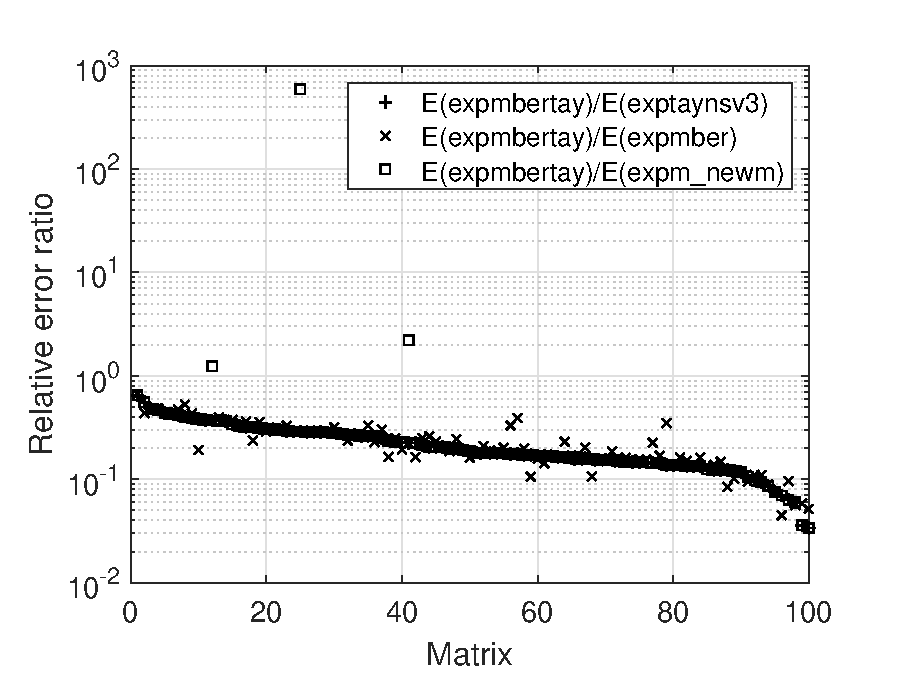
\includegraphics[scale=0.44]{Figures/error_ratio_exp_diag_hadamard_complex_n128_nd256_expmbertay.eps}
\caption{\footnotesize Ratio of relative errors.}
\label{fig:test4_c}
\end{subfigure}
\caption{Experimental results for Test~1.}
\label{fig:test4}
\end{figure}
        
\begin{figure}[t]
\centering
\begin{subfigure}[b]{0.48\textwidth}
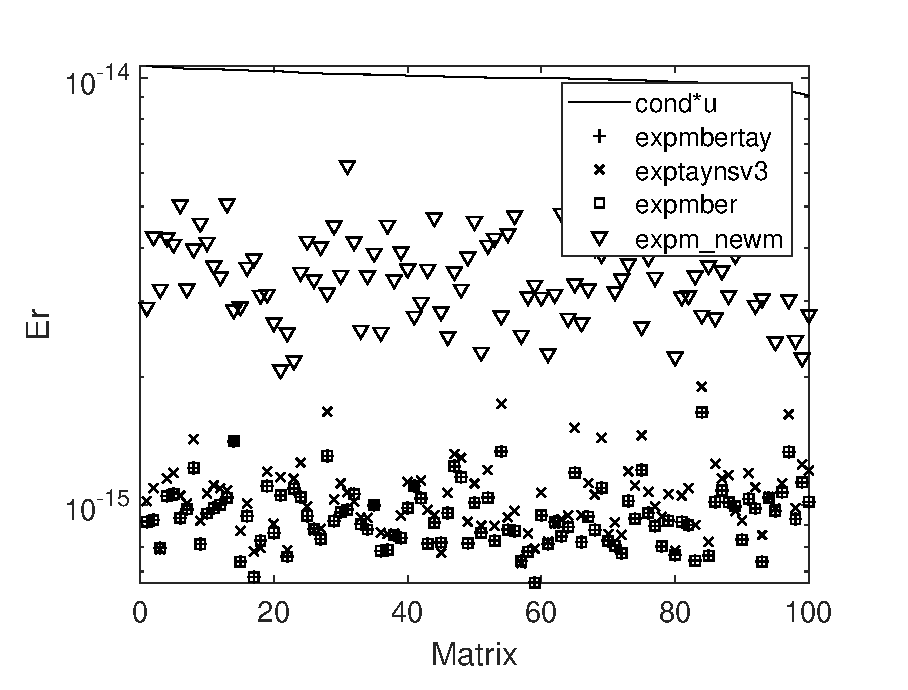
\includegraphics[scale=0.44]{Figures/normwise_exp_jordan_hadamard_complex_n128_boundvp10_maxmult5_nd256_expmbertay.eps}
\caption{\footnotesize Normwise relative errors.} \label{fig:test5_a} \vspace{12pt}
\end{subfigure} \ \
\begin{subfigure}[b]{0.48\textwidth}
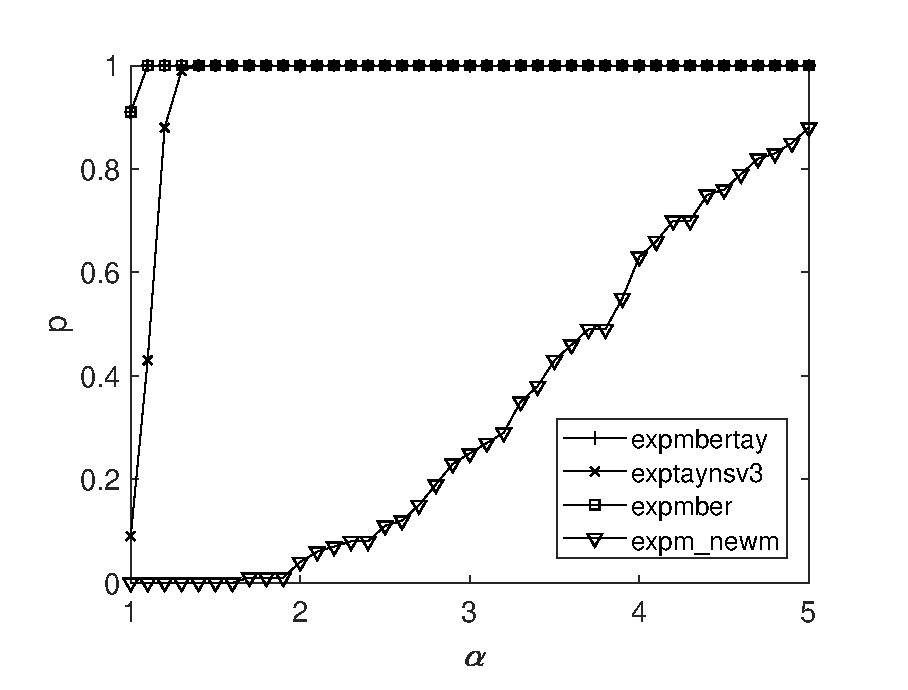
\includegraphics[scale=0.44]{Figures/nprofile_exp_jordan_hadamard_complex_n128_boundvp10_maxmult5_nd256_expmbertay.eps}
\caption{\footnotesize Performance profile.}
\label{fig:test5_b}
\vspace{12pt}
\end{subfigure}
\begin{subfigure}[b]{0.48\textwidth}
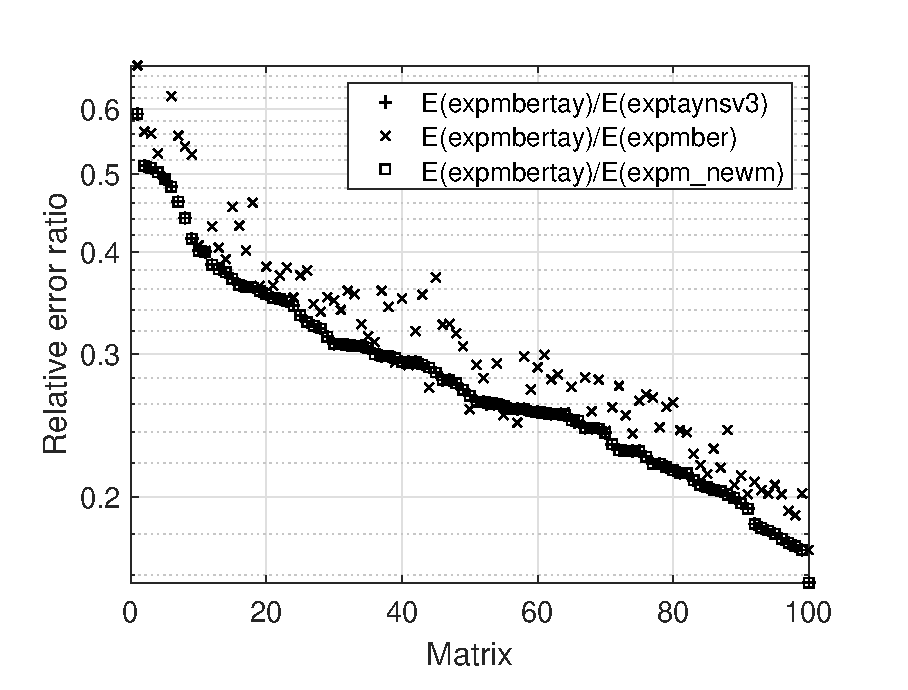
\includegraphics[scale=0.44]{Figures/error_ratio_exp_jordan_hadamard_complex_n128_boundvp10_maxmult5_nd256_expmbertay.eps}
\caption{\footnotesize Ratio of relative errors.}
\label{fig:test5_c}
\end{subfigure}
\caption{Experimental results for Test~2.}
\label{fig:test5}
\end{figure}

\begin{figure}[t]
\centering
\begin{subfigure}[b]{0.48\textwidth}
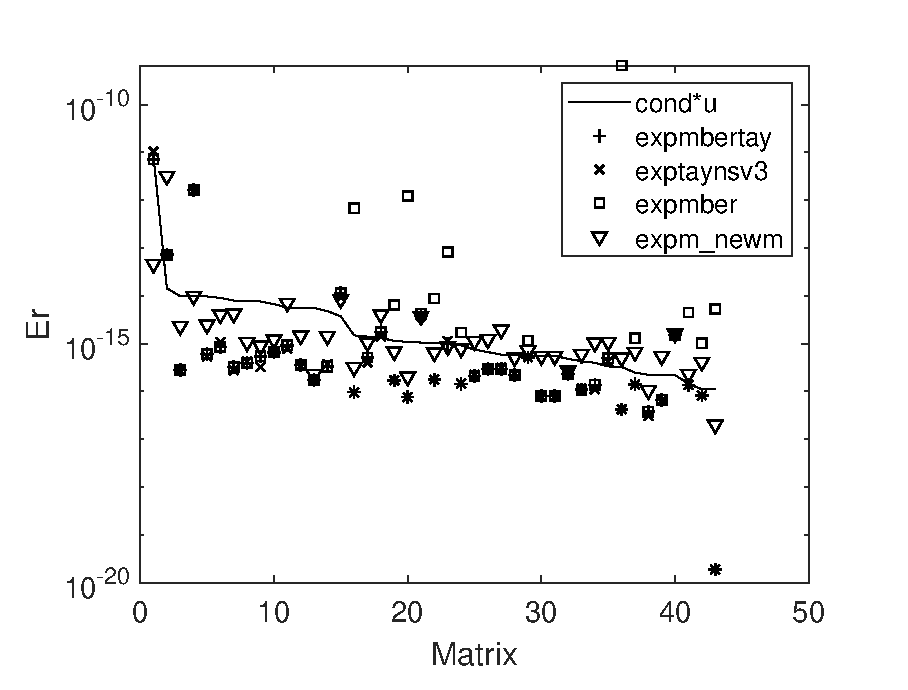
\includegraphics[scale=0.44]{Figures/normwise_exp_toolbox_n128_nd256-exp_eigtool_n128_nd256_expmbertay.eps}
\caption{\footnotesize Normwise relative errors.} \label{fig:test6_a} \vspace{12pt}
\end{subfigure} \ \
\begin{subfigure}[b]{0.48\textwidth}
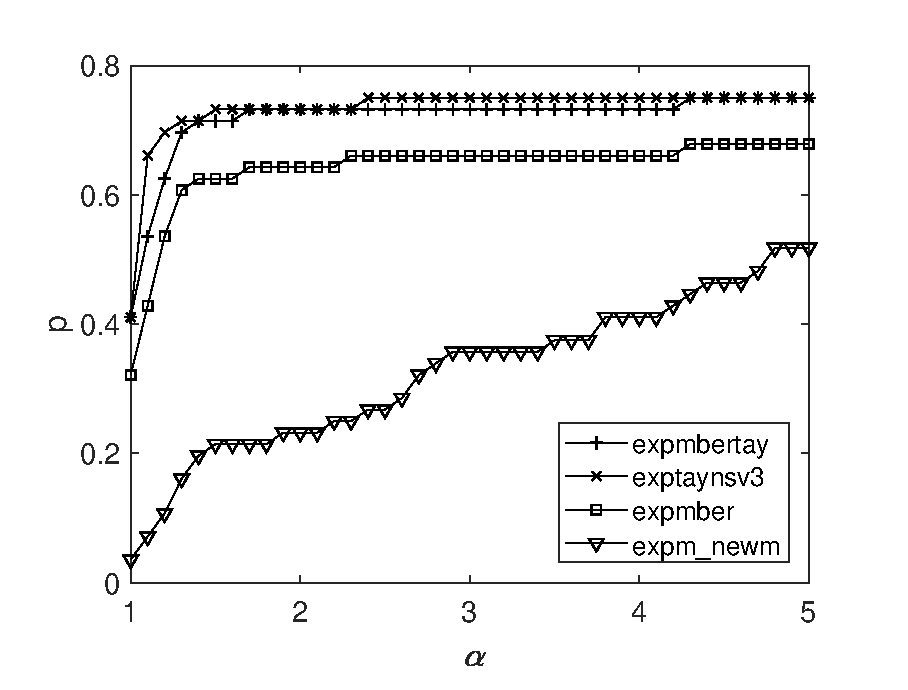
\includegraphics[scale=0.44]{Figures/nprofile_exp_toolbox_n128_nd256-exp_eigtool_n128_nd256_expmbertay.eps}
\caption{\footnotesize Performance profile.}
\label{fig:test6_b}
\vspace{12pt}
\end{subfigure}
\begin{subfigure}[b]{0.48\textwidth}
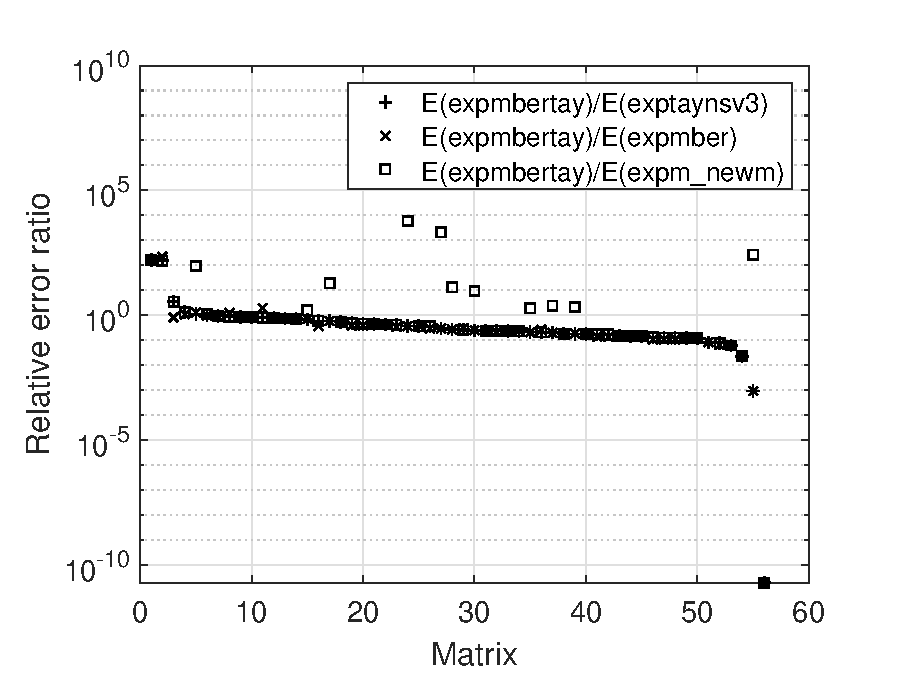
\includegraphics[scale=0.44]{Figures/error_ratio_exp_toolbox_n128_nd256-exp_eigtool_n128_nd256_expmbertay.eps}
\caption{\footnotesize Ratio of relative errors.}
\label{fig:test6_c}
\end{subfigure}
\caption{Experimental results for Test~3.}
\label{fig:test6}
\end{figure}


We have also included in the software developed an ``accelerated'' version of the algorithm proposed in this paper to compute the matrix exponential on an \nvidia\ GPU.
Matrix multiplication is an operation very rich in intrinsic parallelism that can be optimized for GPUs.  
Algorithms, like the one proposed, that rely on many matrix multiplications can be highly get the most of this devices through the use of the cuBLAS~\cite{CuLi09} package.


%Current GPUs are computational devices that allow to boost performance on data parallelism applications, i.e. applications that operate over many independent data.
%This is the case of matrix multiplication, which is a highly optimized operation for GPUs in its current implementation routine included in the cuBLAS~\cite{CuLi09} package.
%%Since our GPU algorithms are all based on Taylor approximations, which are rich in matrix products, we can get the best out of these devices.
%Our GPU algorithms are all based on polynomial evaluations which, in turn, results in intensive use of matrix products. 

Experimental results, shown in Fig.~\ref{fig:results_gpu}, were carried out on a computer equipped with two processors 
Intel Xeon CPU E5-2698 v4 @2.20GHz (\emph{Broadwell} architecture) featuring 20 cores each.
The CPU version execution shown in the figure was obtained using all the 40 cores available in the target computer. 
To get the algorithm performance on the GPU, we used one NVIDIA Tesla P100-SXM2 (\emph{Kepler} architecture) that counts on 3584 CUDA cores and 16 GB of memory.

\begin{figure}[!t]
        \setlength{\tabcolsep}{-10pt}
        \begin{center}
                %\begin{tabular}{cc}
                %\hspace{12pt}
                %\includegraphics[width=0.80\textwidth]{Tiempoparalelo.eps}
                \includegraphics[scale=0.9]{Figures/Tiempoparalelo.eps}
                %\includegraphics[width=0.57\textwidth]{Tflops.eps}
                %\end{tabular}
        \end{center}
        \caption{\label{fig:results_gpu} Execution time (sec.) of the algorithm to compute the matrix exponential using the Taylor series (\texttt{exptaynsv3}) and the Bernoulli (\texttt{expmber}) series on CPU and on GPU for large diagonalizable matrices.}
\end{figure}

At the light of Figure~\ref{fig:results_gpu}, it can be concluded that both the former algorithm based on Taylor series (\texttt{exptaynsv3}) and the one based on Bernoulli series (\texttt{expmber}), studied in this paper, very similarly regarding the execution time, also on the two target architectures tackled: the host CPU and one of the most currently advanced GPUs.  
The reduction in time obtained with the GPU regarding the CPU starts approximately with matrices of size $n=1000$.
The weight of both algorithms falls on the same basic computational kernel (matrix multiplications) and both of them require an identical number of them. The computational performance of routine \texttt{expmbertay} will be very similar to \texttt{expmber}, since it uses once again the same number of matrix products.

\section{Conclusions}
The starting point of this work is a new expression of the exponential matrix cast in terms of Bernoulli matrix polynomials. Using this series expansion, a new method for calculating the exponential of a matrix (implemented as \texttt{expmber} algorithm) has been developed. 
The proposed algorithm has been tested using a state-of-the-art test matrix battery with different features (diagonalizable and non diagonalizable, with particular eigenvalue spectrum) that covers a wide range of cases. The developed code has been compared with the best implementations available, i.e. Pad\'e-based algorithm (\texttt{expm\_new}) and Taylor-based one (\texttt{exptaynsv3}), outperforming Pad\'e-based algorithm and giving results at the level of Taylor-based solutions in both accuracy and computational cost. 

Preliminary results with the Bernoulli version for the exponential matrix function motivated us to develop a hybrid algorithm (called \texttt{expmbertay}) that combines the best of both the Taylor and Bernoulli solutions and resulting in excellent results. Finally, we showed that the two algorithms developed in this contribution keep the advantages of other ones based on matrix polynomial expansion. Since they all are based on matrix multiplications, the GPU version implemented has turned out to be a strong tool to compute the matrix exponential approximation when the numerical methods employed are stressed with large dimension matrices. 

\section*{Acknowledgements}
This work has been partially supported by Spanish Ministerio de Econom\'{\i}a y Competitividad and European Regional Development Fund (ERDF) grants TIN2017-89314-P
and by the Programa de Apoyo a la Investigaci\'on y Desarrollo 2018 of the Universitat Polit\`{e}cnica de Val\`{e}ncia (PAID-06-18) grants SP20180016.

\bibliographystyle{elsarticle-num}
\bibliography{bib_general}
\end{document}
\endinput
%%
%% End of file `elsarticle-template-num.tex'.
